\section{Introducci\'on}
Toda se\~nal enviada por un sistema de comunicaci\'on sufre perturbaciones durante el proceso de transmisi\'on, y es por eso que se desea reducir el error de la informaci\'on recibida.
Un modelo discreto sencillo de un sistema de comunicaciones es el siguiente. Peri\'odicamente, cada T segundos el transmisor env\'ia un dato $s_k$ considerando como instante inicial a $t = 0$. Para los objetivos de este trabajo, se clasifican dos tipos de errores de distinta naturaleza asociados al proceso de transmisi\'on: error sistemático de respuesta impulsiva del canal (el cual depende del medio donde la información se propaga y de la se\~nal), y ruido blanco gaussiano que agrega incertezas que no podemos mejorar. El objetivo entonces es el de recuperar la se\~nal original, teniendo que:
\begin{enumerate}
	\item cuantificar los errores vinculados,
	\item dar un estimador que se aproxime lo más que se pueda a la se\~nal original,
	\item y resolver sistemas de ecuaciones lineales eficientemente para as\'i evitar errores num\'ericos (como redondeo, esto \'ultimo se debe a que la computadora tiene una representaci\'on finita de n\'umeros reales).
\end{enumerate}

 Modelamos el problema como sigue (para sistemas LTI): La informaci\'on es modificada por el canal a través de su "respuesta impulsiva". Esto es la respuesta del sistema (en este caso, el canal) frente a una se\~nal de entrada en particular que se conoce como impulso unitario \'o delta de dirac. Matem\'aticamente, esto permite expresar la salida de un sistema en general como la convoluci\'on de su respuesta impulsiva con la se\~nal de entrada.
A su vez, la señal transmitida es afectada por ruido blanco Gaussiano aditivo , donde $N_k \sim cN(0,\sigma)$. Entonces, peri\'odicamente la informaci\'on recibida es 

\begin{equation*} 
r_n = \sum_{k=0}^{L-1} h_k s_{n-k} + N_n 
\end{equation*} 

Donde $h$  es la respuesta impulsiva previamente mencionada. Matricialmente, esto se puede expresar de dos formas distintas:

\begin{equation}  
\vec{r} = H \vec{s} + \vec{N} 
\label{eq: r=hs+n}
\end{equation} 

\begin{equation} 
\vec{r} = S \vec{h} + \vec{N} 
\label{eq: r=sh+n}
\end{equation} 

Siendo en todos los casos 
\begin{itemize}
	\item \textbf{h} referente a informaci\'on del canal
	\item \textbf{s} referente a información de la se\~nal original
	\item \textbf{n} referente al ruido agregado a la señal
	\item \textbf{r} referente a la se\~nal recibida
\end{itemize}
	
Adem\'as, puede observarse que como la se\~nal recibida es una variable aleatoria, dado que el ruido gaussiano es aleatorio y no hay manera de conocer la respuesta impulsiva con precisi\'on infinita; debe elegirse adecuadamente el estimador de $S_k$ de manera tal de minimizar el error – cuantific\'andose por el m\'etodo de cuadrados m\'inimos de estad\'istica.

\begin{figure}[H]
	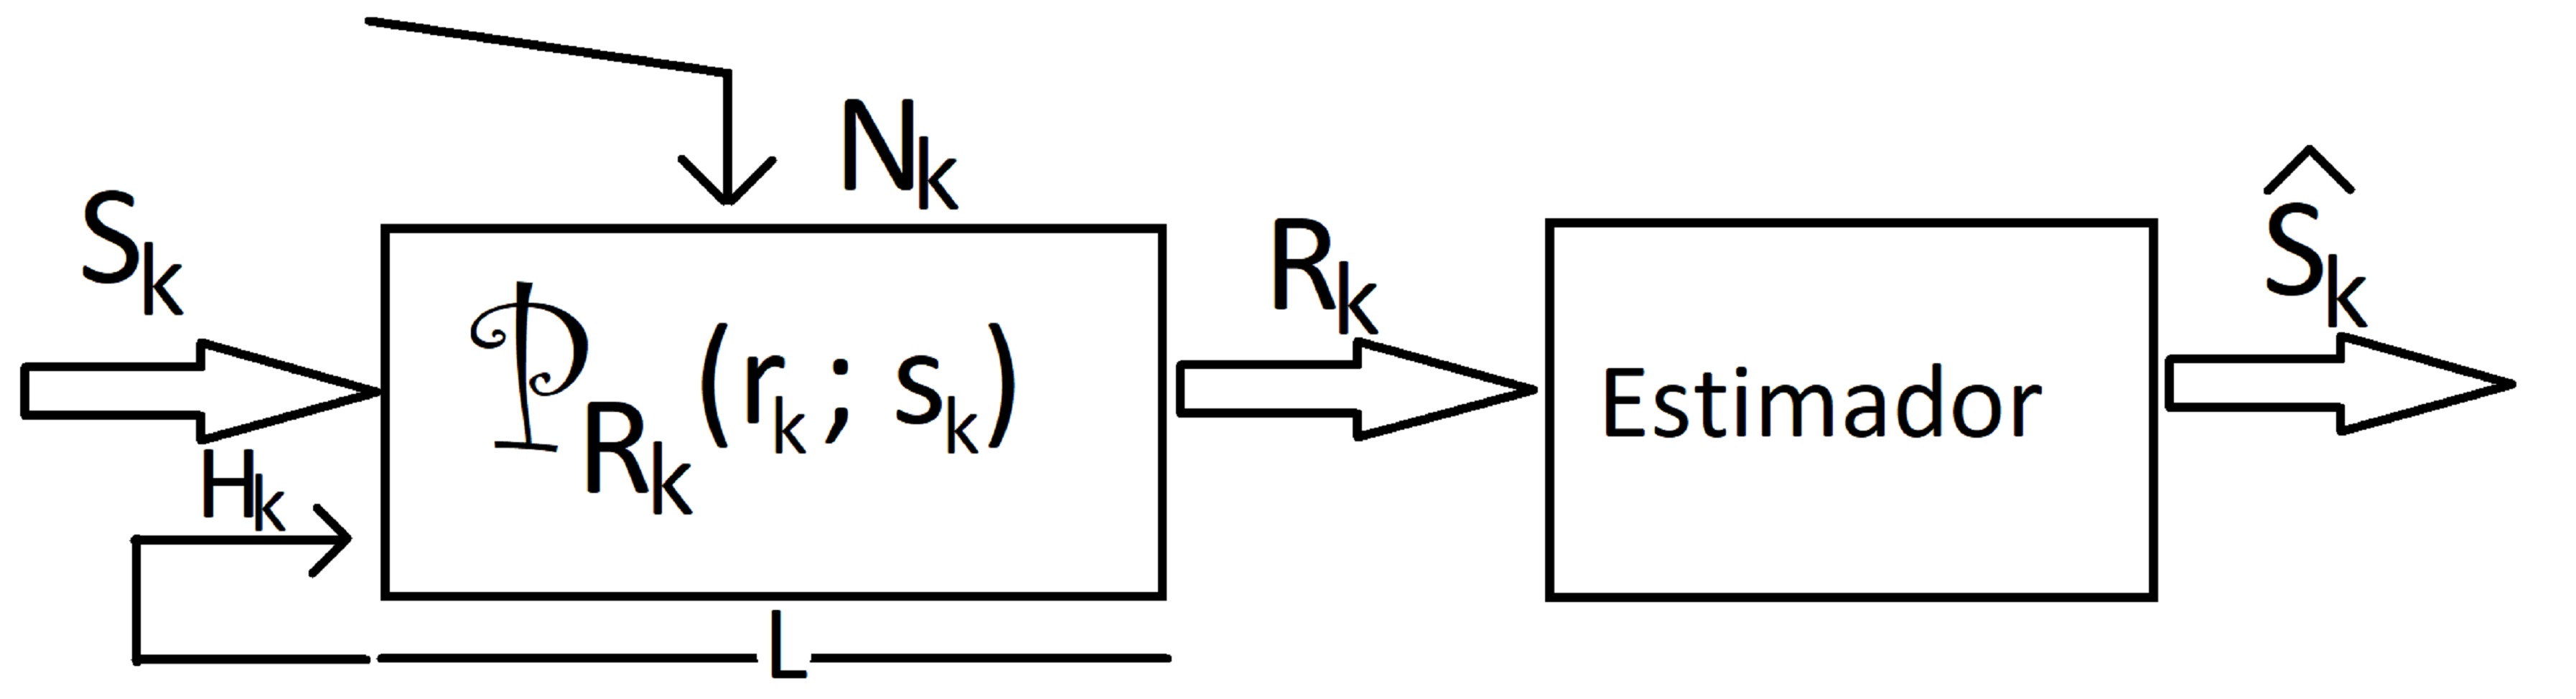
\includegraphics[scale=0.15]{Imagenes/sistema}
	\centering
	\caption {Representaci\'on del sistema y la estimaci\'on de la se\~nal de entrada.}
	\label{sistema}
\end{figure}

Como se puede ver en la Figura \ref{sistema}, se recibe una se\~nal $R_k$ como respuesta a una se\~nal enviada $S_k$. Como el transmisor tiene errores de dos tipos, adem\'as del correspondiente estimador es necesario acotar el error.

%-------------------------------------------------------------------------------------------------------------------------
\section{Estimaci\'on de la se\~nal enviada}

Es necesario hacer una estimaci\'on de dos cosas distintas. Por un lado se debe estimar el canal ($\vec{h}$) y por otro lado, la imagen original  ($\vec{s}$).

%----------------------------------------------
\subsection{Estimaci\'on del canal de comunicaci\'on}

Primero se hace una estimaci\'on de $\vec{h}$ con el m\'etodo de cuadrados m\'inimos, empleando la descomposici\'on de Cholesky, como se explica a continuaci\'on.  Para averiguar $\vec{h}$ a partir de la ecuaci\'on (\ref{eq: r=sh+n}), se busca minimizar:
\begin{equation}
%Min__{h ε R^L} {(S\vec{h} – \vec{r})norma}$ 
%\min_{\forall h \in R^L} S\vec{h} – \vec{r}
\min_{\forall h \in R^L}  || S \vec{h} – \vec{r}  ||
\label{eq: min}
\end{equation}
Por lo que se env\'ia una secuencia conocida de $S$ de prueba para cuantificar el error sistem\'atico impulsivo sobre la se\~nal original. La norma de la ecuaci\'on \ref{eq: min} es norma dos. Se aclara que se realiza una aproximaci\'on, se busca el vector $\vec{h}$ que minimiza ese error — pero como el sistema est\'a influenciado por un proceso estoc\'astico nunca se va a hallar la respuesta impulsiva exacta (que depende del material y de la se\~nal enviada).
Teniendo esto \'ultimo en cuenta, consideramos entonces la ecuaci\'on:


%se considera que la media del ruido $N$ es cero, y as\'i se obtiene una nueva ecuaci\'on a partir de la cu\'al se proceder\'a:

\begin{equation} 
\vec{r} = S \vec{h}
\label{eq: r=sh} 
\end{equation} 

Para utilizar el m\'etodo de Cholesky en una ecuaci\'on del tipo $\vec{b} = A \vec{h}$ es necesario que la matriz $A$ sea cuadrada, sim\'etrica y definida positiva. Pero en nuestro caso,  en su lugar tenemos a la matriz $S$, que como se observa en la ecuación \ref{eq: r=sh+n} es triangular inferior y no es cuadrada. Como necesitamos una matriz que cumpla estas condiciones, multiplicamos ambos lados de la ecuaci\'on (\ref{eq: r=sh}) por $S^T$:

\begin{equation} 
S^T \vec{r} = S^T S \vec{h} 
\end{equation} 

Llamamos  $S^T \vec{r} = \vec{b}$ y  $S^T S = A$, y obtenemos la expresi\'on:

\begin{equation} 
\vec{b} = A \vec{h} 
\label{eq: b=Ah} 
\end{equation} 

En esta nueva ecuaci\'on (\ref{eq: b=Ah}), la matriz A la conforma el producto que $S^T$ por $S$, por lo que ahora además de ser cuadrada, la norma usual definida por la matriz $S S^T$ es siempre mayor a cero dado que los bits de Lena resultan ser as\'i. Por consiguiente, se cumplen las hipótesis de Cholesky y $A$ es definida positiva para toda señal que se escriba de la forma que previamente se definió en el marco teórico del sistema. Para implementar este m\'etodo, el cual consiste en encontrar las matrices $L$ y $L^T$ triangulares, tales que $A = L L^T$, para simplificar la resoluci\'on de la ecuaci\'on. Una vez averiguadas las matrices  $L$ y $L^T$,en la ecuaci\'on (\ref{eq: b=Ah}) reemplazamos la matriz $A$ por el producto entre ellas y obtenemos:

\begin{equation} 
\vec{b} = L L^T \vec{h} 
\label{eq: b=LLth}
\end{equation} 

Llamamos $\vec{y} = L^T \vec{h}$ y lo reemplazamos en la ecuaci\'on (\ref{eq: b=LLth}), de modo que:

\begin{equation} 
\vec{b} = L \vec{y}
\label{eq: b=Ly}
\end{equation} 

A partir de la ecuaci\'on (\ref{eq: b=Ly}) obtenemos $ \vec{y}$ realizando sustituci\'on Forward. Finalmente, dado que, como se mencion\'o previamente:

 \begin{equation} 
\vec{y} = L^T \vec{h} 
\label{eq: y=Lth}
\end{equation}

se despeja $\vec{h}$ de la ecuaci\'on (\ref{eq: y=Lth}) haciendo una sustituci\'on Backward. La ventaja de implementar el m\'etodo de Cholesky para la ecuaci\'on resuelta es que se terminan resolviendo dos ecuaciones en las que la matriz involucrada (ya sea $L$ o $L^T$) es una matriz triangular.

%----------------------------------------------
\subsection{Estimaci\'on de la imagen original}
Una vez usada la secuencia de entrenamiento para tener un estimador para la respuesta impulsiva H, se procede a minimizar el error cuadrático medio del estimador de la imagen de Lena. La estimaci\'on de la imagen original $\vec{s}$, se hace a partir de la ecuaci\'on (\ref{eq: r=hs+n}), de una manera distinta a la implementada para la estimaci\'on de  $\vec{h}$. A pesar de que tambi\'en se realiza haciendo cuadrados m\'inimos, asumimos que el nivel de ruido es conocido y usamos otro m\'etodo  conocido como Linear Minimum Square Error (LMMSE); donde las deducciones de las f\'ormulas que se usan para hallar el estimador vienen de plantear una suerte de regresi\'on lineal; y luego buscar maximizar la probabilidad seg\'un Maximum Likelihood Estimation (si se modela con Estad\'istica Cl\'asica o Frecuentista) o Maximum a Posteriori Probability Estimation (si se modela con Estad\'istica Bayesiana).  Si bien no es lo correcto, asumimos que las m\'inimas unidades transmitidas en la se\~nal enviada son independientes entre s\'i, simplemente para que la resoluci\'on sea m\'as sencilla. 

Para ver c\'omo funciona todo lo explicado hasta aqu\'i, se env\'ia la imagen de Lena con un ruido de un desv\'io est\'andar que se va variando para cada experimento,, y para dos valores de $E$ distintos. Siendo $E$ la longitud de la secuencia de entrenamiento. A continuaci\'on se observan los resultados de la transmisi\'on de la imagen de Lena en escala de grises.

\begin{figure}[H]
	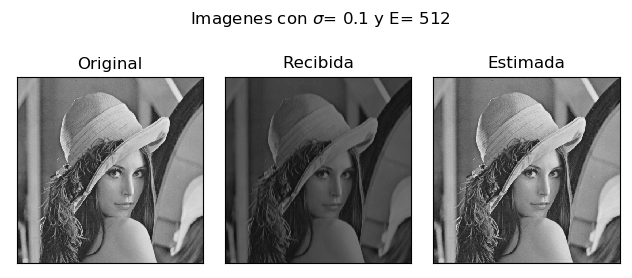
\includegraphics[scale=1.5]{Imagenes/1}
	\centering
\end{figure}

\begin{figure}[H]
	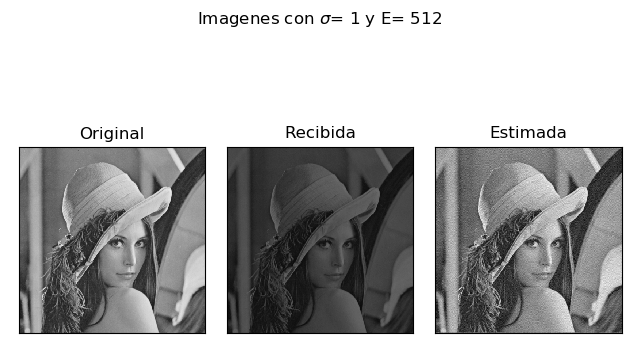
\includegraphics[scale=1.5]{Imagenes/2}
	\centering
\end{figure}
 
\begin{figure}[H]
	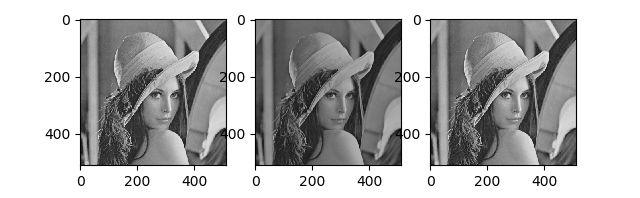
\includegraphics[scale=1]{Imagenes/E32S00}
	\centering
\end{figure}

\begin{figure}[H]
	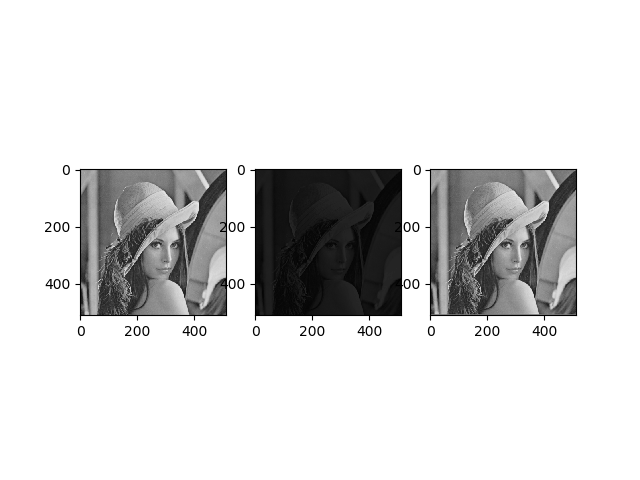
\includegraphics[scale=1]{Imagenes/E32S01}
	\centering
\end{figure}
 
\begin{figure}[H]
	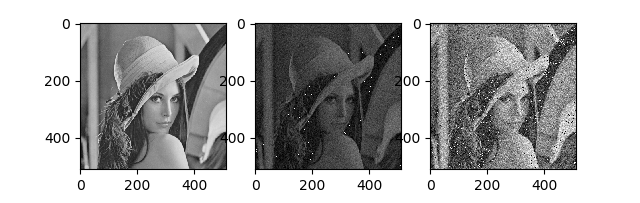
\includegraphics[scale=1]{Imagenes/E32S10}
	\centering
\end{figure}

\begin{figure}[H]
	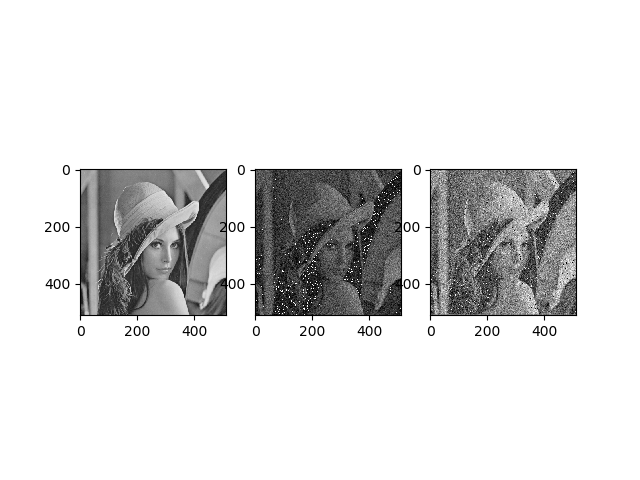
\includegraphics[scale=1]{Imagenes/E32S20}
	\centering
\end{figure}

\begin{figure}[H]
	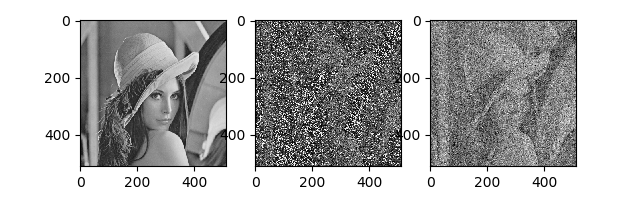
\includegraphics[scale=1]{Imagenes/E32S50}
	\centering
\end{figure}

\begin{figure}[H]
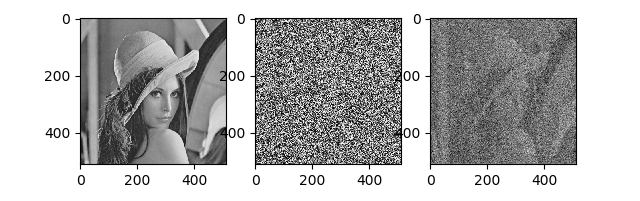
\includegraphics[scale=1]{Imagenes/E32S100}
\centering
\end{figure}

\begin{figure}[H]
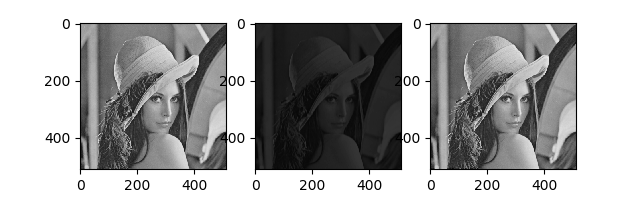
\includegraphics[scale=1]{Imagenes/E1024S00}
\centering
\end{figure}

\begin{figure}[H]
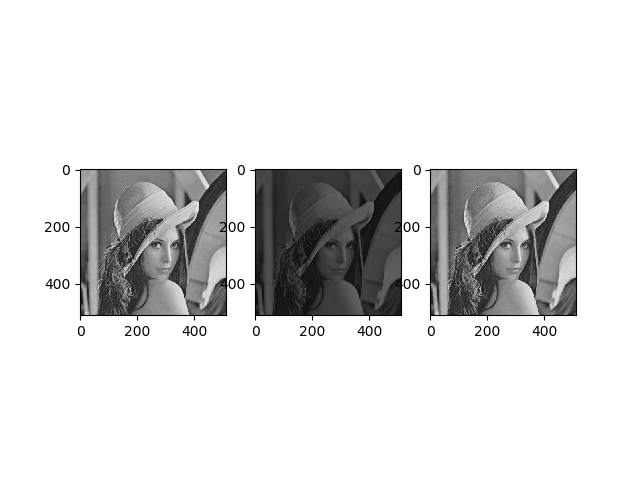
\includegraphics[scale=1]{Imagenes/E1024S01}
\centering
\end{figure}

\begin{figure}[H]
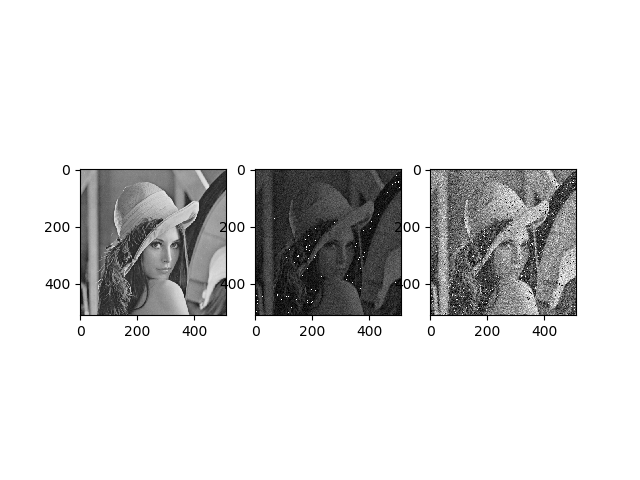
\includegraphics[scale=1]{Imagenes/E1024S10}
\centering
\end{figure}

\begin{figure}[H]
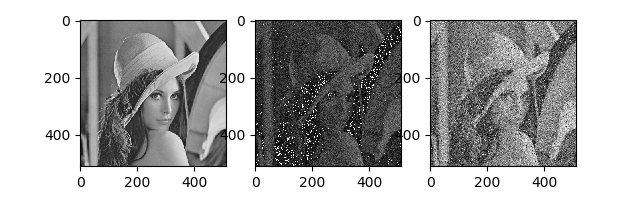
\includegraphics[scale=1]{Imagenes/E1024S20}
\centering
\end{figure}

\begin{figure}[H]
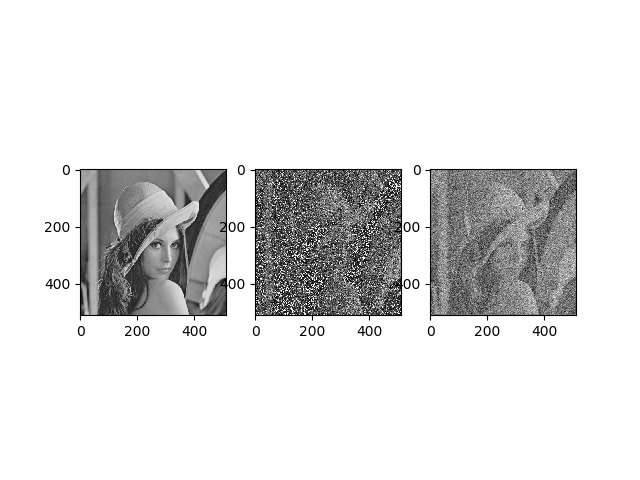
\includegraphics[scale=1]{Imagenes/E1024S50}
\centering
\end{figure}

\begin{figure}[H]
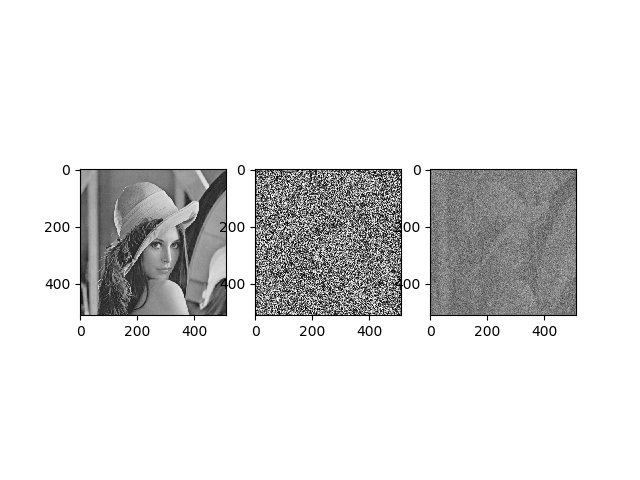
\includegraphics[scale=1]{Imagenes/E1024S100}
\centering
\end{figure}

%explicar los resultados haciendo comparaciones entre los resultados y la imagen real, y entre los resultados y el ruido y entre los resultados distintos debiedo a la variable que se fue cambiando.

\section{Conclusi\'on - An\'alisis de im\'agenes}
Tras ascender la desviaci\'on est\'andar del ruido gaussiano, provoca que el estimador resultante sea muy distinto respecto de la se\~nal original. Aunque los efectos impulsivos se puedan cuantificar con una se\~nal de prueba, estos no est\'an aislados del ruido Gaussiano, y por ende genera desviaciones agregadas adem\'as del $N_k$ en s\'i que son dif\'iciles de solventar, aun asumiendo conocido el nivel de ruido. La ventaja entonces del uso de la se\~nal de entrenamiento es aprovecharse del hecho de que, como la respuesta impulsiva $h_k$ depende del medio de comunicaci\'on (con su par\'ametro de longitud) y la se\~nal que con cada experimento no cambia (enti\'endase por experimento a cuando se genera un solo h particular, que vendr\'ia a estar asociado a cambiar el medio y la se\~nal), quiere decir que $h_k$ es determinista y el aporte aleatorio viene dado por $N_k$. Esto explica el efecto de por qu\'e tras aumentar la cantidad de informaci\'on, $E$, no afecta demasiado en comparaci\'on a cambiar el desv\'io est\'andar del ruido gaussiano, por lo menos en el rango estudiado. Sí puede apreciarse de todas maneras, que acrecentar el $E$ conlleva a aumenta el error cuadr\'atico medio y por ende la imagen original tiende a distinguirse a\'un m\'as de la recuperada por el estimador. 

\section{Anexo}
A continuaci\'on se presenta el c\'odigo empleado para realizar las estimaciones y graficar las imagenes de este trabajo. 
Aclaraci\'on: en utils.py se encuentran las funciones que hab\'ia que implementar. Se adjuntan tambi\'en los .py del c\'odigo que se muestran a continuaci\'on. En caso de ejecutarlo, es necesario correr ej1.py teniendo en el mismo directorio utils.py y lena.bmp.


\begin{lstlisting}[language=Python, caption=Ej1.py]
from utils import *
from numpy import *
from numpy.random import *
from matplotlib.pyplot import *
from scipy.linalg import toeplitz
from numpy.linalg import inv

E = 32
sigma = 0.1
L = 5
ganancia = 1/10
h = ganancia*(1+randn(1,L))
a = imread(("lena512.bmp"))
M = len(a[:, 0])
P = len(a[0, :])
z = np.zeros(M-L)
H = toeplitz(np.concatenate((h,z),axis=None),zeros(M))
r = zeros((M,P))
N = sigma*randn(M,P)
s = a.astype(float64)
r = matmul(H,s) + N
b = uint8(r)
# #------------------------------

sE = np.random.uniform(1,255,size=(E,1))-1
ME= len(sE[:, 0]) #cols
PE= len(sE[0, :]) # fils
#ajusto sE para el producto

HE= toeplitz(concatenate((h,zeros(ME-L)),axis=None),zeros(ME))
rE= zeros((ME,PE))
NE= sigma*randn(ME,PE)
rE = matmul(HE,sE) + NE
S = toeplitz(sE.transpose())

#S = S(:,1:L) # en octave dame todas las columnas de 1 a L
S= S[:,0:L+1] # en python 0:L+1 incluye hasta L

S = tril(S)
# multiplicamos ambos miembros por izquierda para obtener una matriz
# simetrica y aplicar cholesky
St = S.transpose()

he=solveEq(matmul(St,S),matmul(St,rE))

#comparo h con hE
compareh= [h,he]
print(compareh)
He= toeplitz(concatenate((he,zeros(M-L-1)),axis=None),zeros(M))

CN= (sigma**2)*eye(len(He))

sigmax= (1/256*(sum(np.power (((range(0,255))-mean(range(0,255))),2))))**(1/2)
mx= mean(range(0,255))*ones(M)
CX= (sigmax**2)*eye(len(He))

aux = matmul(matmul(He,CX),He.transpose())+CN
W = matmul(matmul(CX,He.transpose()),inv(aux))
#----------------------------------------------------------

d = zeros((M,P))
for k in range(0,P):
    #d(:,k) accede en octave a la columna k-esima
    d[:, k] = W.dot((r[:, k])-He.dot(mx)) + mx

d = uint8(d)


#graficamos

figure(2)

suptitle("Imagenes con $\sigma$= "+str(sigma)+" y E= "+str(E))

subplot(1,3,1)
imshow(a,cmap='gray',vmin=0,vmax=255)
yticks([])
xticks([])
title("Original")

subplot(1,3,2)
yticks([])
xticks([])
imshow(b,cmap='gray',vmin=0,vmax=255)
title("Recibida")

subplot(1,3,3)
imshow(d,cmap='gray',vmin=0,vmax=255)
yticks([])
xticks([])
title("Estimada")
tight_layout()
name = "E" + str(E) + "S" + str(sigma)
show()
\end{lstlisting}
---------------------------------------------------------------------------------------------------------------------------------------------------
%%%%%%%%%%%%%%%%%%%%%
\begin{lstlisting}[language=Python, caption=utils.py]
import numpy as np

def cholesky(a):
    #esta funcion asume que a es es semidefinida positiva y simetrica
    #(esto esta justificado en el informe)
    w = len(a)
    l = np.zeros((w,w)) # matriz de wxw
    #sum1 y sum2 son las sumatorias de las formulas
    sum1 = 0
    sum2 = 0
    #j es columna,i es fila
    #como lo primero que termina una iteracion en el proceso son las filas
    #entonces deben estar adentro del for de las columnas
    for j in range(0, w):
        for i in range(j, w):
            if i == j: #formula para cuando i vale j
                for k in range(0, i):
                    sum1 += (l[i][k]) ** 2
                l[i][i] = (a[i][i] - sum1) ** (1 / 2)
                sum1 = 0
            else:     #formula para cuando i distinto j
                for k in range(0, j):
                    sum2 += l[i][k]*l[j][k]
                l[i][j] = (a[i][j]-sum2)/(l[j][j])
                sum2 = 0
    return l

def backSubs(u,y):
    # queremos resolver u x = y
    # con a triangular superior
    n = len(u)
    x = np.zeros(n)
    sum = 0
    for i in range(n-1,-1,-1): # [n-1,0]
        for j in range(i+1,n):
            sum += x[j]*u[i][j]
        x[i]=(y[i]-sum)/u[i][i]
        sum = 0
    return x

def ForwSubs(u,y):
    # queremos resolver u x = y
    # con u triangular inferior
    n=len(u)
    x =np.zeros(n)
    sum = 0
    for i in range(0,n): # n a 1
        for j in range(0,i):
            sum += x[j]*u[i][j]
        x[i]=(y[i]-sum)/u[i][i]
        sum = 0
    return x


def solveEq(a,b):
    #solve ax = b
    #hacemos cholesky
    L = cholesky(a)
    #primero resolvemos L y = b
    y = ForwSubs(L,b)
    #luego resolvemos (L)t x = y
    x = backSubs(L.transpose(),y)
    return x
\end{lstlisting}

